% Propósito: visualizar la tendencia logarítmica de la ley de masas y sus límites.
% Origen: R_masa = 20 log10(m f) + constante; duplicar m o f suma
% 20 log10(2) = 6,02 dB. No se usan datos de materiales.
% Accesibilidad: dos rectas paralelas para masas m y 2m suben con la frecuencia;
% una llave muestra 6,02 dB y se señalan regiones no descritas por el modelo.
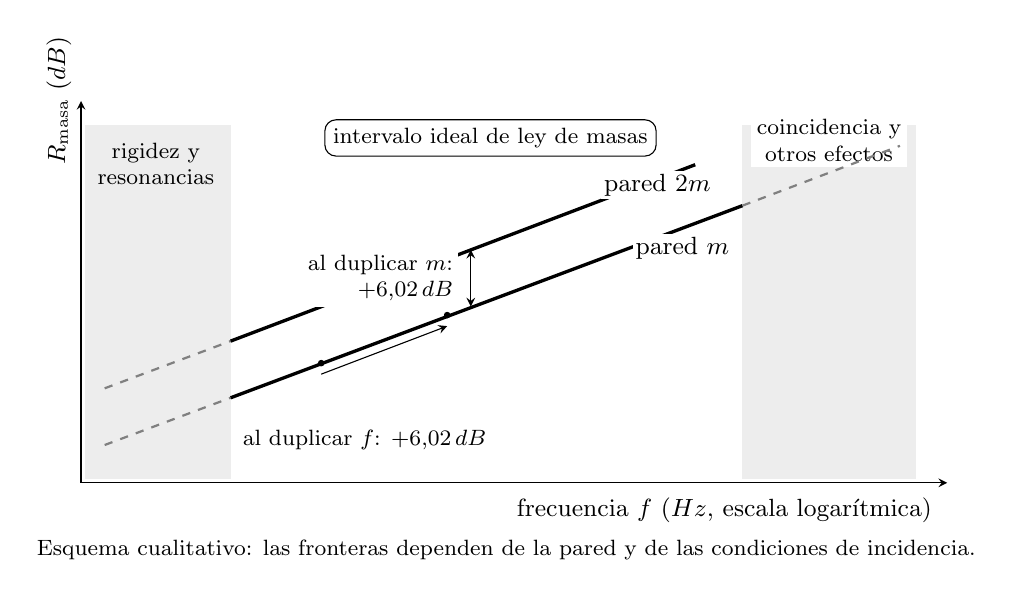
\begin{tikzpicture}[
    x=1cm,
    y=1cm,
    >=stealth,
    font=\small,
    ideal/.style={very thick},
    fuera/.style={thick,gray,dashed}
]
    \draw[->] (1.15,0.70) -- (12.15,0.70)
        node[below left=2pt,font=\small] {frecuencia \(f\) (\(\text{Hz}\), escala logarítmica)};
    \draw[->] (1.15,0.70) -- (1.15,5.55)
        node[above left,rotate=90,anchor=south,font=\small]
        {\(R_\mathrm{masa}\) (\(\text{dB}\))};

    \path[fill=black!7] (1.20,0.75) rectangle (3.05,5.25);
    \path[fill=black!7] (9.55,0.75) rectangle (11.75,5.25);
    \node[align=center,font=\footnotesize] at (2.10,4.75)
        {rigidez y\\resonancias};
    \node[align=center,font=\footnotesize,fill=white,inner sep=2pt]
        at (10.65,5.05)
        {coincidencia y\\otros efectos};

    % Pared de masa m
    \draw[fuera] (1.45,1.18) -- (3.05,1.78);
    \draw[ideal] (3.05,1.78) -- (9.55,4.22);
    \draw[fuera] (9.55,4.22) -- (11.55,4.98);
    \node[anchor=west,fill=white,inner sep=1pt] at (8.15,3.68)
        {pared \(m\)};

    % Pared de masa 2m
    \draw[fuera] (1.45,1.90) -- (3.05,2.50);
    \draw[ideal] (3.05,2.50) -- (8.95,4.74);
    \node[anchor=west,fill=white,inner sep=1pt] at (7.75,4.48)
        {pared \(2m\)};

    % Cambio por duplicar la masa, a frecuencia fija
    \draw[<->] (6.10,2.94) -- (6.10,3.66);
    \node[anchor=east,align=right,font=\footnotesize,fill=white,inner sep=2pt]
        at (5.95,3.30)
        {al duplicar \(m\):\\\(+6{,}02\,\text{dB}\)};

    % Cambio por duplicar la frecuencia sobre una misma recta
    \fill (4.20,2.22) circle (1.2pt);
    \fill (5.80,2.83) circle (1.2pt);
    \draw[->] (4.20,2.08) -- (5.80,2.69);
    \node[align=center,font=\footnotesize,fill=white,inner sep=1pt]
        at (4.75,1.25) {al duplicar \(f\): \(+6{,}02\,\text{dB}\)};

    \node[draw,rounded corners,fill=white,inner sep=3pt,font=\footnotesize]
        at (6.35,5.08) {intervalo ideal de ley de masas};
    \node[font=\footnotesize,anchor=north] at (6.55,0.10)
        {Esquema cualitativo: las fronteras dependen de la pared y de las condiciones de incidencia.};
\end{tikzpicture}
